\chapter{Software}
This project consist mostly of software and experimenting with different configuration to produce the best result. This chapter will enlighten the implementation and also the usage of the driver in the API section.

\section{Quick Setup}
The whole project is available at \url{https://mygit.th-deg.de/nb20429/linux-kernel-driver}. User who has access to the git repository can clone the project or download the repository on the website provided to test the drivers. These are the steps to try the drivers.

\begin{enumerate}
	\item Download or clone the drivers. To download the driver, go to the github repository page and click download button. To clone refer to following webpage \url{https://docs.gitlab.com/ee/gitlab-basics/start-using-git.html#clone-a-repository}
	\item Enter the Code folder and open a terminal. Run following command below to clean and rebuild the drivers including inserting module into kernel.
	\item Run the app to see the temperature displayed on SH1107 using the command below.
\end{enumerate}

\begin{verbatim}
bash driver.sh 0
bash driver.sh 1
./app
\end{verbatim}

\section{Implementation}
This section will explain clearly how each of the driver is implemented. The driver file is written in C as both linux and windows are written in C making C as native language to program a driver. These drivers are then compiled into modules using a tool chain called GNU Compiler Collection (gcc) \url{http://gcc.gnu.org/}. GNU also provide assembler, linker, library and object manipulation tools \cite{barry_chapter_2012}.\\

A module must comprise with an Initialization and Cleanup functions \cite{rubini_linux_2001} which can be implemented on Linux using following these lines of codes:

\begin{verbatim}
module_init(my_init)
module_exit(my_cleanup)
\end{verbatim}

\verb'my_init' and \verb'my_clenup' are any functions you want amodule to run when it is inserted and remove respectively. At the end of each driver file, there must be these lines of codes to give the description to the module:

\begin{lstlisting}[language=C]
MODULE_LICENSE("GPL");
MODULE_AUTHOR("Your Name");
MODULE_DESCRIPTION("GPIO Driver");
MODULE_VERSION("1.0");
\end{lstlisting}

with above mentioned characteristics, one should be able to create the driver. Next subsections will show how each of the drivers are implemented.

\subsection{I2C Driver}
This paper will not discuss the whole codes but the algorithm and data structure of the drivers. It is important to note that the devices use I2C for interfacing communication with Raspberry Pi and therefore will need to use the Linux I2C library. These is stated in the header of every driver.\\
Each module has a common file operations structure as followings~\cite{noauthor_character_nodate}:

\begin{lstlisting}
static const struct file_operations fops =
    {
        .owner = THIS_MODULE,
        .open = dev_open,
        .release = dev_release,
        .read = dev_read,
        .write = dev_write
	};
\end{lstlisting}

This means every driver has specific function for read and write. Furthermore several I2C variables need to be configured as followings in every driver~\cite{noauthor_character_nodate}:

\begin{lstlisting}

static struct i2c_adapter *temp_i2c_adapter = NULL;
static struct i2c_client *temp_i2c_client = NULL;
static const struct i2c_device_id device_id[] = {{SLAVE_DEVICE_NAME, 0},{}};
static struct i2c_driver temp_driver = {.driver = {.name = SLAVE_DEVICE_NAME, .owner = THIS_MODULE}};
static struct i2c_board_info i2c_board_info = {I2C_BOARD_INFO(SLAVE_DEVICE_NAME, SLAVE_ADDRESS)};

\end{lstlisting}

\subsection{Initialization and Cleanup}
The source code for TMP102 and SH1107 driver is in file \verb'temp_driver.c' and \verb'display_driver.c' respectively. As a character device there are necessary steps need to be followed to properly initialize it.

\begin{enumerate}
	\item Allocate character device region.
	\item Initialize character device with file operations mentioned above.
	\item Register device with its number.
	\item Create a class in \verb'/sys/class'
	\item Populate \verb'/sys/sysfs' with device info
\end{enumerate}

After character device has properly configured, I2C communication also must be configured. The steps are stated below.

\begin{enumerate}
	\item Assign I2C adapters with an adapter at available I2C bus
	\item Assign I2C client as new I2C client device
	\item Add I2C driver to the susystem
	\item Release asscociated memory of adapter
\end{enumerate}

After the module removed, it is important that the memory allocation for the character device is carefully cleaned and unregistered. This is to avoid any concurrency of memory for future use. The following steps are necessary in \verb'dev_exit' function.

\begin{enumerate}
	\item Unregister I2C device client
	\item Delete driver from the subsystem
	\item Destroy Character device
	\item Destroy Class associated with the device
	\item Delete the character device
	\item Unregister allocated character device region
\end{enumerate}

\section{TMP102}
TMP102 is an Input device which means that the read function must be configured for the device. The read function retrieves temperature data from the TMP102 sensor. It uses I2C communication to read the temperature bytes from the sensor. The received bytes are combined to form a 16-bit integer value representing the temperature. The integer and decimal parts of the temperature are calculated and formatted as a string. The formatted string is then copied to the user space buffer. Finally, the function returns the number of bytes successfully copied.

\section{SH1107}
SH1107 has more complicated implementation compare to TMP102 as it has multiple configuration and special commands before some text can be written on it. Its Write function receives parameters including the file pointer, a buffer containing the data to be written, the number of bytes to write, and the current file offset.

Within the function, there is a maximum length set for the data, which is initially set to 30 bytes but may be adjusted depending on the value of count. The function then attempts to copy the data from the user space buffer into a local buffer. The number of bytes not copied is checked to determine if the copy was successful. \\ Afterward, the last element of data buf is set to null character to ensure it is a valid string. The function then calls the SH1107 String function to display the string on the SH1107 OLED display. \\
Finally, the function returns the number of bytes written to indicate the success of the operation or any error that may have occurred.

There are unique function associated with SH1107 that has been implemented so that it is able to write text on the display comfortably. These functions will explain in next subsections.

\subsection{SH1107 DisplayInit}
This function initializes the SH1107 OLED display. It sends a series of commands via I2C communication to configure the display settings such as:

\begin{enumerate}
	\item 0xAE: turning it off 
	\item 0xA0: setting the segment re-map and common output scan direction 
	\item 0xC0: setting the display mode to normal
	\item 0xA6: setting the memory addressing mode
	\item 0xAF: finally turning on the display
\end{enumerate}

Additional commands can be read from SH1107 Datasheet~\cite{SH1107_datasheet}

\subsection{SH1107 Fill}
This function fills the entire display with a specific data value. It uses nested loops to iterate over each page and column of the display and sends the data value to each pixel using the SH1107 Write function.

\subsection{SH1107 Write}
This function is responsible for sending commands or data to the SH1107 display via I2C communication. It takes two parameters: \verb'is_cmd' indicates whether the data is a command or display data, and data is the actual command or data value. The function constructs a two-byte buffer with the appropriate command data prefix and then calls the I2C Write function to send the buffer over I2C.
This function will call \verb|I2C_Write()| function which is to send data using I2C protocol. The drawing algorithm is as following.

\begin{enumerate}
	\item The data sent are written in hexadecimal in a char array with a size of 2
	\item The first data byte is intepreted whether it is a command or ram data.  When the byte is equal to 0x40, the inputs at D7 - D0 are interpreted as data and be written to display RAM.
	\item When the byte is equal to 0x00, the inputs at D7 - D0 are interpreted as command, they will
	be decoded and be written to the corresponding command registers.
	\item The second byte are the data or a value that should be written.
	\item The Display Data RAM is a bit mapped static RAM holding the bit pattern to be displayed. The size of the RAM is 128 X 128 bits.
	For mechanical flexibility, re-mapping on segment and the direction of common outputs can be selected by software.
	\item This driver used the page address circuit. The page address must be specified first before writing the data.
	\item The next column is automatically adressed with each display data read/write command in vertical addressing mode.
	\item As example a to write as example in \ref{fig:fig1}, The first byte for ram data should be 0xFF indicating \verb|1111 1111|.
	\item The next byte should be  10001000 an so on.
\end{enumerate}

\begin{figure}
	\centering
	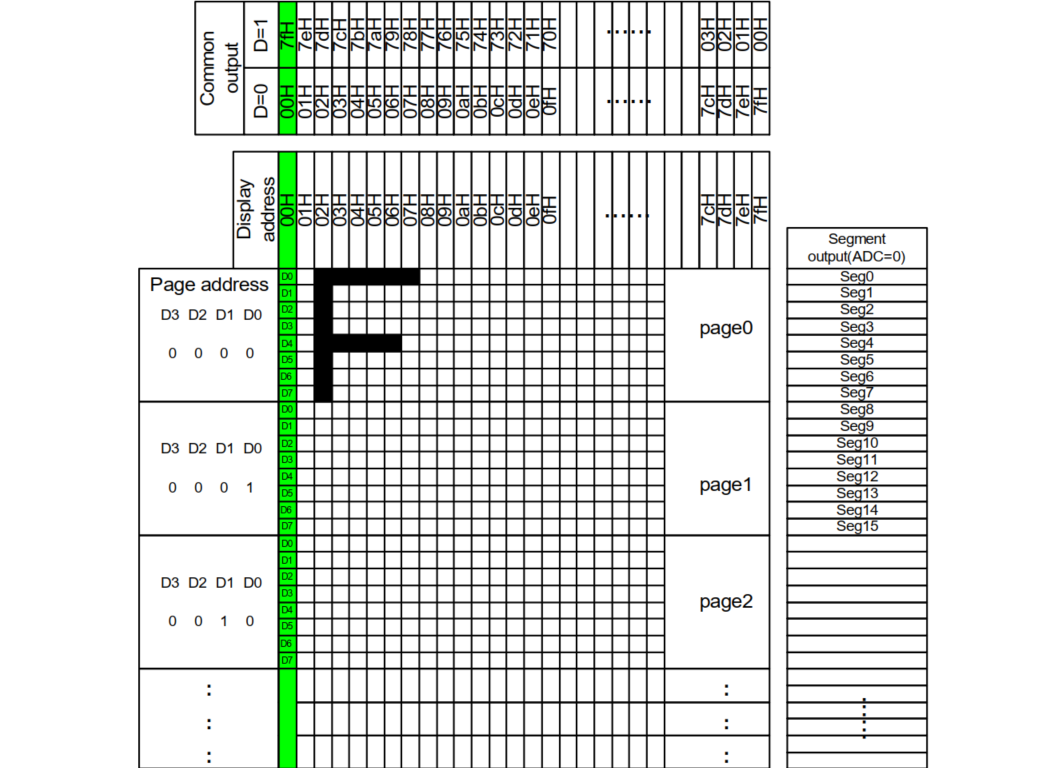
\includegraphics[width=.8\linewidth]{sh1107ram.png}
	\caption{letter ``F'' is written on the ram display}\label{fig:fig1}
\end{figure}

\subsection{SH1107 SetCursor}
This function sets the cursor position on the display. It takes two parameters: lineNo specifies the line number of the display, and cursorPos specifies the cursor position. The function sends the necessary commands to set the page and column addresses using the SH1107 Write function.

\subsection{SH1107 String}
This function displays a string of characters on the SH1107 display. It takes a pointer to a null-terminated string as input. The function iterates over each character in the string and calls the SH1107 PrintChar function to display each character.

\subsection{SH1107 PrintChar}
This function displays a single character on the SH1107 display. It takes a character as input and converts it to the corresponding index in the font table SH1107 font. The function then retrieves the font data for the character and sends it to the display using the SH1107 Write function. It also handles line breaks and backspace characters to manage the cursor position and line wrapping.

\subsection{SH1107 ReturnToFirstSegment}
This function returns the cursor to the beginning of the current line (page) on the display. It fills the remaining segment with zero values using the SH1107 Write function to clear any remaining display data.

\subsection{SH1107 GoToNextLine}
This function moves the cursor to the beginning of the next line on the display. It increments the line number and wraps it around if it exceeds the maximum line value. It then calls SH1107 ReturnToFirstSegment to clear the segment before displaying new data.